\documentclass{beamer}
\usepackage[utf8]{inputenc}
\usepackage{amsthm}
\usepackage{tikz}
\usepackage{circuitikz}
\usetikzlibrary{arrows, positioning}
\usepackage{algorithmic}
\usepackage{tabularx}

\usepackage{amsmath}
\usepackage[utf8]{inputenc}
\usepackage{amsmath}  % For advanced mathematical typesetting
\usepackage[ruled,vlined]{algorithm2e}  % For writing algorithms
\usetikzlibrary{calc}
% \usetikzlibrary{crypto.symbols}
\usetikzlibrary {positioning}
\usetikzlibrary{shapes}

\usetikzlibrary{arrows, positioning}
% Referance
\usepackage[backend=biber]{biblatex}
\addbibresource{main.bib}

\usepackage{listings}
\usepackage{xcolor}
\lstset{
  language=Python,
  basicstyle=\ttfamily\small,
  keywordstyle=\color{blue},
  commentstyle=\color{gray},
  stringstyle=\color{orange},
  numbers=left,
  numberstyle=\tiny\color{gray},
  stepnumber=1,
  numbersep=5pt,
  breaklines=true,
  showstringspaces=false,
  tabsize=4
}
\setbeamertemplate{caption}[numbered]

\usetheme{Madrid}
\usecolortheme{default}

%------------------------------------------------------------
%This block of code defines the information to appear in the
%Title page
\title[MILP IN
CRYPTANALYSIS ] %optional
{USAGE OF MIXED INTEGER
LINEAR PROGRAMMING IN
CRYPTANALYSIS OF BLOCK
CIPHERS}


\author[Halil İbrahim Kaplan] % (optional)
{Halil İbrahim Kaplan }

\institute[] % (optional)
{
  Istanbul Technical University\\
  Informatics Institute
}

\date[2025] % (optional)
{2025}



%End of title page configuration block
%------------------------------------------------------------



%------------------------------------------------------------
%The next block of commands puts the table of contents at the 
%beginning of each section and highlights the current section:

\AtBeginSection[]
{
  \begin{frame}
    \frametitle{Table of Contents}
    \tableofcontents[currentsection]
  \end{frame}
}
%------------------------------------------------------------


\begin{document}

%The next statement creates the title page.
\frame{\titlepage}


%---------------------------------------------------------
%This block of code is for the table of contents after
%the title page
\begin{frame}
\frametitle{Table of Contents}
\tableofcontents
\end{frame}
%---------------------------------------------------------
\section{Preliminaries}

\begin{frame}{Block Ciphers}
    Block ciphers are main elements in symmetric cryptography, designed to securely
encrypt and decrypt fixed-size blocks of data by transforming plaintext into ciphertext
using a symmetric key. 
k   

Figure ekle!!!!
\end{frame}

\begin{frame}{Block Cipher types}

    \begin{figure}[H]
        \centering
        % Private Key Table
        \begin{minipage}{0.45\textwidth}
        \centering
        \includegraphics[width=1.2\linewidth]{fig/spn.png}
        \caption{SPN Cipher}
        \label{fig:SPN}
        \end{minipage}
        \hfill
        % Public Key Table
        \begin{minipage}{0.45\textwidth}
        \centering
        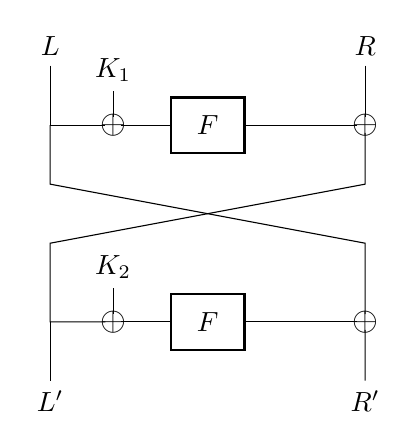
\begin{tikzpicture}[auto,transform shape]
    \tikzstyle{block} = [rectangle, draw, thick,
        text width=2em, text centered, minimum height=2em]
    \tikzstyle{line} = [draw, -]
    
    \node [block] (Et) {$F$};
    \coordinate [above of=Et, node distance=1cm] (top);
    \coordinate [left of=Et, node distance=2cm] (midleft);
    \node [left of=top, node distance=2cm] (m1) {$L$};
    \node [left of=Et, node distance=1.2cm, thick, scale=1.2] (xor1) {$\mathbf{\oplus}$};
    \node [above of=xor1, node distance=0.7cm] (4L1) {$K_{1}$};
    \coordinate [left of=xor1, node distance=1mm] (xor11);
    \path [line] (m1) -- (midleft) -- (xor11);
    \coordinate [above of=xor1, node distance=1mm] (xor12);
    \path [line] (4L1) -- (xor12);
    \coordinate [right of=xor1, node distance=1mm] (xor13);
    \path [line] (xor13) -- (Et);
    %
    \node [right of=top, node distance=2cm] (m2) {$R$};
    \node [right of=Et, node distance=2cm, thick, scale=1.2] (xor2) {$\mathbf{\oplus}$};
    \coordinate [left of=xor2, node distance=1mm] (xor21);
    \path [line] (Et) -- (xor21);
    \coordinate [above of=xor2, node distance=1mm] (xor22);
    \path [line] (m2) -- (xor22);
    %
    \coordinate [below of=midleft, node distance=.75cm] (botleft);
    \coordinate [below of=botleft, node distance=.75cm] (bumleft);
    \coordinate [right of=botleft, node distance=4cm] (botright);
    \coordinate [right of=bumleft, node distance=4cm] (bumright);
    \coordinate [below of=xor2, node distance=1mm] (xor23);
    \node [block, below of=Et, node distance=2.5cm] (Eb) {$F$};
    %
    \coordinate [left of=Eb, node distance=2cm] (bimleft);
    \node [left of=Eb, node distance=1.2cm, thick, scale=1.2] (xor3) {$\mathbf{\oplus}$};
    \coordinate [left  of=xor3, node distance=1mm] (xor31);
    \coordinate [above of=xor3, node distance=1mm] (xor32);
    \coordinate [right of=xor3, node distance=1mm] (xor33);
    \coordinate [below of=xor3, node distance=1mm] (xor34);
    \node [above of=xor3, node distance=0.7cm] (4L2) {$K_{2}$};
    %
    \path [line] (xor23) -- (botright) -- (bumleft) -- (bimleft) -- (xor31);
    \path [line] (4L2) -- (xor32);
    \path [line] (xor33) -- (Eb);
    %
    \node [right of=Eb, node distance=2cm, thick, scale=1.2] (xor4) {$\mathbf{\oplus}$};
    \coordinate [below of=xor4, node distance=1mm] (xor41);
    \coordinate [left of=xor4, node distance=1mm] (xor42);
    \coordinate [above of=xor4, node distance=1mm] (xor43);
    \path [line] (midleft) -- (botleft) -- (bumright) -- (xor43);
    \path [line] (Eb) -- (xor42);
    %
    \node [below of=m1, node distance=4.5cm] (c1) {$L'$};
    \node [right of=c1, node distance=4cm] (c2) {$R'$};
    \path [line] (bimleft) -- (c1);
    \path [line] (xor41) -- (c2);
    
    \end{tikzpicture}
    \caption{Fiestel Structure}
    \label{fig:fiestel}
        \end{minipage}
        
    \end{figure}
    
\end{frame}
\begin{frame}{Cryptanalysis}

    The main
purpose of cryptanalysis is to prove that an algorithm is secure against known attacks
in the open literature or find better complexities for those attacks and contribute to the
security of the algorithm. In cryptanalysis, breaking an algorithm means obtaining the
key with a lower complexity than the algorithm claims.
    
\end{frame}

\begin{frame}[t]{AES-128 Security Against Cryptanalytic Attacks}
\footnotesize % Reduce font size to fit table
\setlength{\tabcolsep}{4pt} % Reduce column spacing
\begin{tabularx}{\textwidth}{|l|X|X|X|l|}
\hline
\textbf{Attack Type} & \textbf{Best Known Result} & \textbf{Complexity (Time / Data)} & \textbf{Full 10-Round AES-128} & \textbf{Reference} \\
\hline
Brute Force & Exhaustive key search & $2^{128}$ time, negligible data & Infeasible & \cite{daemen2002rijndael} \\
\hline
Linear Cryptanalysis & Works up to 7 rounds & $\approx 2^{126.1}$ time, $\approx 2^{126.1}$ data & No distinguisher & \cite{matsui1993linear,daemen2002rijndael} \\
\hline
Differential Cryptanalysis & Works up to 7 rounds & $\approx 2^{126.1}$ time, $\approx 2^{126.1}$ data & No distinguisher & \cite{biham1991differential,daemen2002rijndael} \\
\hline
Impossible Differential & Attacks up to 6 rounds & $\approx 2^{110}$ time, $\approx 2^{110}$ data & Not effective & \cite{biryukov2009related} \\
\hline
Integral (Square) Attack & Effective up to 6--8 rounds & $\approx 2^{124}$ time, full codebook data & No attack & \cite{daemen1997square,ferguson2000algebraic} \\
\hline
Related-Key Attacks & Attacks up to 9 rounds & $2^{99.5}$ time, $2^{32}$ related keys & No single-key break & \cite{biryukov2009related} \\
\hline
Algebraic Attacks & Solve AES equations via Gröbner basis & $>2^{128}$ time & Not effective & \cite{courtois2002cryptanalysis} \\
\hline
\end{tabularx}
\end{frame}

\section{LP and MILP}
%---------------------------------------------------------
\begin{frame}{Linear Programming}
The standard form of a linear programming (LP) problem is:

\vspace{0.5em}
\textbf{Maximize (or Minimize):}
\begin{align*}
    c_1x_1 + c_2x_2 + \dots + c_nx_n
\end{align*}

\vspace{0.5em}
\textbf{Subject to:}
\begin{align*}
    a_{11}x_1 + a_{12}x_2 + \dots + a_{1n}x_n &\leq b_1 \\
    a_{21}x_1 + a_{22}x_2 + \dots + a_{2n}x_n &\leq b_2 \\
    &\vdots \\
    a_{m1}x_1 + a_{m2}x_2 + \dots + a_{mn}x_n &\leq b_m \\
    x_1, x_2, \dots, x_n &\geq 0
\end{align*}

\vspace{0.5em}
\small
Here, $x_1, x_2, \dots, x_n$ are the \textbf{decision variables}, $c_1, c_2, \dots, c_n$ are the \textbf{coefficients of the objective function}, $a_{ij}$ are the \textbf{constraint coefficients}, and $b_1, b_2, \dots, b_m$ are the \textbf{constraint bounds}.
\end{frame}
%---------------------------------------------------------
\begin{frame}{Mixed-Integer Linear Programming}
Mixed-Integer Linear Programming (MILP) extends LP by requiring some variables to take integer values:

\vspace{0.5em}
\textbf{Maximize (or Minimize):}
\begin{align*}
    c_1x_1 + c_2x_2 + \dots + c_nx_n
\end{align*}

\vspace{0.5em}
\textbf{Subject to:}
\begin{align*}
    a_{11}x_1 + a_{12}x_2 + \dots + a_{1n}x_n &\leq b_1 \\
    a_{21}x_1 + a_{22}x_2 + \dots + a_{2n}x_n &\leq b_2 \\
    &\vdots \\
    a_{m1}x_1 + a_{m2}x_2 + \dots + a_{mn}x_n &\leq b_m \\
    x_1, x_2, \dots, x_p &\in \mathbb{Z} \\
    x_{p+1}, x_{p+2}, \dots, x_n &\geq 0
\end{align*}

\vspace{0.5em}
\small
In this formulation, the first $p$ decision variables ($x_1, x_2, \dots, x_p$) must be \textbf{integers}, while the remaining $n-p$ variables ($x_{p+1}, \dots, x_n$) are \textbf{real-valued}.
\end{frame}

%---------------------------------------------------------
\begin{frame}{MILP example}

A company produces two types of products, \textbf{Product A} and \textbf{Product B}. The goal is to maximize profit while considering production capacity, resource availability, and a minimum production requirement. The constraints involve available labor hours, machine hours, and minimum production levels.

\end{frame}
%---------------------------------------------------------
\begin{frame}{MILP example}
    \textbf{Variables:} \linebreak
    
    \begin{itemize}
        \item $x$ be the number of units produced of \textbf{Product A}.
        \item $y$ be the number of units produced of \textbf{Product B}.
    \end{itemize}
    
    Both $x$ and $y$ are integer variables.\linebreak
    
    \textbf{Objective Function:} \linebreak
    
    Maximize the total profit:
    $
    \text{Maximize} \quad Z = 40x + 30y
    $
    where:
    \begin{itemize}
        \item 40 is the profit per unit of \textbf{Product A},
        \item 30 is the profit per unit of \textbf{Product B}.
    \end{itemize}
    
\end{frame}
%---------------------------------------------------------
\begin{frame}{MILP example}
    \textbf{Constraints}
    \begin{enumerate}
        \item \textbf{Labor Constraint}: Each unit of \textbf{Product A} requires 2 hours of labor, and each unit of \textbf{Product B} requires 1 hour of labor. The total available labor hours are 100.
        $
        2x + y \leq 100
        $
        
        \item \textbf{Machine Hours Constraint}: Each unit of \textbf{Product A} requires 1 hour of machine time, and each unit of \textbf{Product B} requires 3 hours of machine time. The total available machine hours are 90.
        $
        x + 3y \leq 90
        $
        
        \item \textbf{Minimum Production Constraint}: At least 20 units of \textbf{Product A} must be produced to meet market demand.
        $x \geq 20$
        
        \item \textbf{Non-Negativity Constraint}: The number of units produced cannot be negative.
        $x \geq 0, \quad y \geq 0$
    \end{enumerate}
    
\end{frame}
%---------------------------------------------------------
\begin{frame}[fragile]{MILP example}
We will use Sagemath and GLPK solver for modeling Toy example. After running the below code, we found that Maximum profit 2160 can be achieved by producing  42 A product and 16 B product. \\

\begin{lstlisting}
p.<x,y> = MixedIntegerLinearProgram(maximization=True, solver="GLPK")
p.set_objective(40*x[0] + 30*y[0])
p.add_constraint(2*x[0] + y[0] == 100)
p.add_constraint(x[0] + 3*y[0] == 90)
p.add_constraint(x[0] >= 20)
p.add_constraint(y[0] >= 0)
print(p.solve())
print(p.get_values(x, y))
\end{lstlisting}
    
\end{frame}
%---------------------------------------------------------
\begin{frame}{MILP example}
\begin{center}
    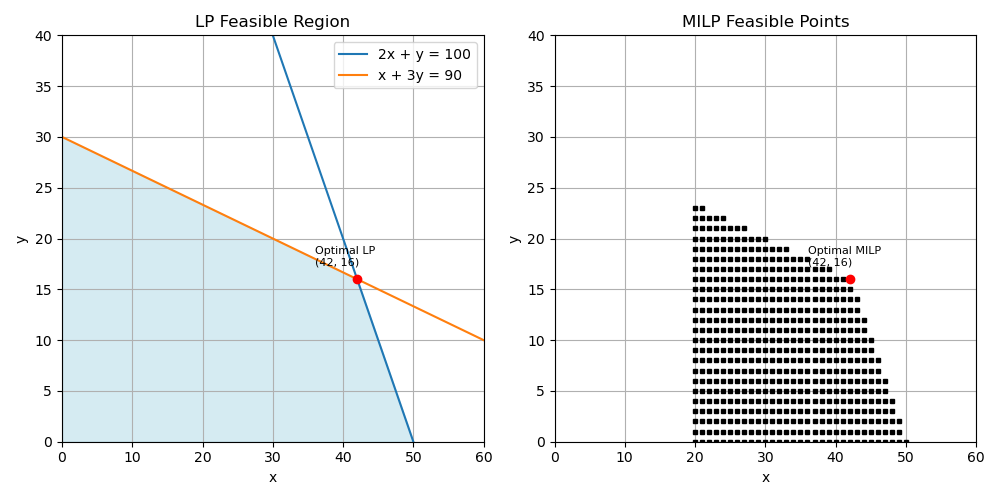
\includegraphics[width=\linewidth]{fig/lp_milp_example.png}
\end{center}
    
\end{frame}
%---------------------------------------------------------
\section{Differential Cryptanalysis}
%---------------------------------------------------------
\begin{frame}{Differential Cryptanalysis}
    Differential cryptalysis is chosen plaintext attack founded by Bilham and Shamir
against Data Encryption Standart (DES) Once the effectiveness of the attack against
DES was seen, it became standard to apply differential attacks to demonstrate the
security of all block cipher algorithms.
\end{frame}
%---------------------------------------------------------
\begin{frame}
\frametitle{Differential Cryptanalysis}

\begin{block}{Definition}
Assume that $P$ and $P'$ two plaintexts then difference $\Delta P$ is defined as 
  $ \Delta P = P \oplus P' $
\end{block}

Differential Cryptanalysis leverages the high probability of specific plaintext differences $\Delta X$ and the differences in the cipher's final round $\Delta Y$. 
\end{frame}
%---------------------------------------------------------
\begin{frame}
\frametitle{Differential Cryptanalysis}

 In an ideal cipher:
\begin{itemize}

    \item For a given $\Delta X$, the probability that a specific $\Delta Y$ occurs is $1/2^n$ (where n is the number of bits in X).

    \item Differential Cryptanalysis aims to find instances where, for a given $\Delta X$, the probability of a specific $\Delta Y$ occurring is significantly higher or lower than $1/2^n$.
    
\end{itemize}
\end{frame}
%---------------------------------------------------------
\begin{frame}
\frametitle{Differential Cryptanalysis}

    \begin{block}{Definition}
    Diff characteristic is sequence of input and output differences to the rounds so that the output difference from one round corresponds to the input difference for the next round.
    \end{block}
    
    \vspace{1 em}
    In order to construct differential characteristic for the cipher we need to find differential for each round with very high or low occurrences. To find thees characteristics we need to examine the nonlinear parts of the cipher like s-boxes. To examine the s-boxes, we use difference distribution tables (DDT)
    
\end{frame}
%---------------------------------------------------------
\begin{frame}
\frametitle{Differential Cryptanalysis}

\begin{figure}
    \centering
    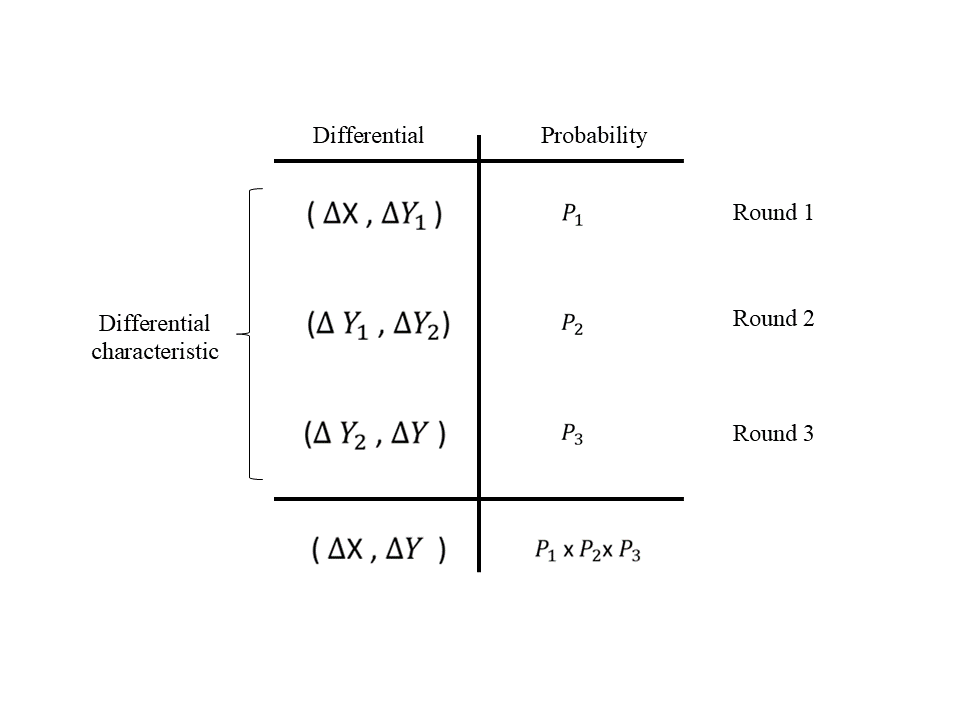
\includegraphics[width=0.8\linewidth]{fig/difchar.png}
    \caption{Concept of constructing differential characteristic}
    \label{fig:difchar}
\end{figure}

\end{frame}
%---------------------------------------------------------
\begin{frame}
\frametitle{Differential Cryptanalysis}

    \begin{block}{Definition}
    DDT is a matrix that tabulates the number of occurrences of specific output differences $(\Delta Y)$ for each possible input difference $(\Delta X)$ after a single round of a cipher.
    \end{block}

    \vspace{1 em}
    \begin{algorithm}[H]
        \DontPrintSemicolon
        Initialize an empty DDT table \\
            \For{$0 \leq dx < 2^{n}-1$}{
                \For {$0 \leq x < 2^{n}-1$}{ 
                    $x1 = dx \oplus x$ \\                    
                    $y = sbox(x)$ \\                  
                    $y1 = sbox(x1)$ \\                    
                    $dy = y \oplus y1 $ \\                    
                    $DDT[dx][dy] += 1$ \\      
                }
            }
        \caption{Pseudocode for DDT }
        \label{alg:ddtkod}
    \end{algorithm}
    \vspace{2 em}
    
\end{frame}
%---------------------------------------------------------
\begin{frame}
\frametitle{Differential Cryptanalysis}


\begin{table}[h!]
\centering
\footnotesize
\begin{tabular}{|c|c|c|c|c|c|c|c|c|c|c|c|c|c|c|c|c|}
\hline
$\Delta X / \Delta Y $ & 0 & 1 & 2 & 3 & 4 & 5 & 6 & 7 & 8 & 9 & A & B & C & D & E & F \\
\hline
0 & 16 & 0 & 0 & 0 & 0 & 0 & 0 & 0 & 0 & 0 & 0 & 0 & 0 & 0 & 0 & 0 \\
\hline
1 & 0 & 0 & 0 & 0 & 0 & 0 & 0 & 0 & 4 & 4 & 4 & 4 & 0 & 0 & 0 & 0 \\
\hline
2 & 0 & 4 & 0 & 4 & 0 & 4 & 4 & 0 & 0 & 0 & 0 & 0 & 0 & 0 & 0 & 0 \\
\hline
3 & 0 & 0 & 0 & 0 & 0 & 0 & 0 & 0 & 2 & 2 & 2 & 2 & 2 & 2 & 2 & 2 \\
\hline
4 & 0 & 0 & 4 & 0 & 0 & 0 & 2 & 2 & 0 & 0 & 0 & 4 & 2 & 2 & 0 & 0 \\
\hline
5 & 0 & 0 & 4 & 0 & 0 & 0 & 2 & 2 & 0 & 0 & 4 & 0 & 2 & 2 & 0 & 0 \\
\hline
6 & 0 & 2 & 0 & 2 & 2 & 0 & 0 & 2 & 2 & 0 & 2 & 0 & 0 & 2 & 2 & 0 \\
\hline
7 & 0 & 2 & 0 & 2 & 2 & 0 & 0 & 2 & 0 & 2 & 0 & 2 & 2 & 0 & 0 & 2 \\
\hline
8 & 0 & 0 & 0 & 0 & 4 & 4 & 0 & 0 & 0 & 0 & 0 & 0 & 2 & 2 & 2 & 2 \\
\hline
9 & 0 & 0 & 0 & 0 & 4 & 4 & 0 & 0 & 0 & 0 & 0 & 0 & 2 & 2 & 2 & 2 \\
\hline
A & 0 & 0 & 0 & 0 & 0 & 4 & 4 & 0 & 2 & 2 & 2 & 2 & 0 & 0 & 0 & 0 \\
\hline
B & 0 & 4 & 0 & 4 & 0 & 0 & 0 & 0 & 0 & 0 & 0 & 0 & 2 & 2 & 2 & 2 \\
\hline
C & 0 & 0 & 4 & 0 & 0 & 0 & 2 & 2 & 4 & 0 & 0 & 0 & 0 & 0 & 2 & 2 \\
\hline
D & 0 & 0 & 4 & 0 & 0 & 0 & 2 & 2 & 0 & 4 & 0 & 0 & 0 & 0 & 2 & 2 \\
\hline
E & 0 & 2 & 0 & 2 & 2 & 0 & 0 & 2 & 0 & 2 & 0 & 2 & 0 & 2 & 2 & 0 \\
\hline
F & 0 & 2 & 0 & 2 & 2 & 0 & 0 & 2 & 2 & 0 & 2 & 0 & 2 & 0 & 0 & 2 \\
\hline
\end{tabular}
\caption{Differential Distribution Table (DDT) of PRINCE algorithm}
\label{tbl:ddtprince}
\end{table} 
    
\end{frame}
%---------------------------------------------------------
\begin{frame}
\frametitle{Differential Cryptanalysis}

    \begin{enumerate}
    \item \textbf{Selection of Differentials:}
    \begin{itemize}
        \item Identify differentials $(\Delta X, \Delta Y)$ with non-random propagation probabilities by examining the cipher's S-boxes using the Differential Distribution Table (DDT).
        \item Select differentials with the highest probabilities for the analysis.
    \end{itemize}

    \item \textbf{Collection of Pairs:}
    \begin{itemize}
        \item Obtain a large number of plaintext pairs $(P, P')$ such that $P \oplus P' = \Delta X$.
    \end{itemize}

    \item \textbf{Cipher Execution:}
    \begin{itemize}
        \item Encrypt the selected plaintext pairs through the cipher.
    \end{itemize}

\end{enumerate}
    
\end{frame}
%---------------------------------------------------------
\begin{frame}
\frametitle{Differential Cryptanalysis}

    \begin{enumerate}
    \setcounter{enumi}{3} % Continue numbering from 4
    \item\textbf{Analysis of Output Differences:}
    \begin{itemize}
        \item Analyze the differences in the output ciphertext pairs.
        \item Check if the observed differences match the expected $\Delta Y$.
    \end{itemize}

    \item \textbf{Key Recovery:}
    \begin{itemize}
        \item Use the observed differentials and the associated probabilities to guess parts of the encryption key, focusing particularly on the subkeys used in the last few rounds.
    \end{itemize}
    \end{enumerate}
    
\end{frame}
%---------------------------------------------------------

\section{ITUbee Block Cipher}

%---------------------------------------------------------
\begin{frame}
\frametitle{ITUbee Block Cipher}
\begin{figure}[!ht]
\centering
\resizebox{1\textwidth}{!}{%
\begin{circuitikz}
\tikzstyle{every node}=[font=\Large]

\node [font=\Large] at (2.5,16) {PL};
\draw (2.5,15.5) to[short] (2.5,14.5);
\draw  (2.5,14) circle (0.5cm);
\draw [short] (2.5,13.5) -- (2.5,11.5);
\draw [->, >=Stealth] (2.5,11.5) -- (4,11.5);
\draw  (4,12) rectangle  node {\large F} (5.25,11);
\draw [->, >=Stealth] (5.25,11.5) -- (6.5,11.5);
\draw [short] (2.5,14.5) -- (2.5,13.5);
\draw [short] (2,14) -- (3,14);
\draw  (7,11.5) circle (0.5cm);
\draw [->, >=Stealth] (7.5,11.5) -- (8.75,11.5);
\draw  (11.25,12) rectangle  node {\Large L} (12.5,11);
\draw [->, >=Stealth] (12.5,11.5) -- (14,11.5);
\draw  (14,12) rectangle  node {\Large F} (15.25,11);
\draw [->, >=Stealth] (15.25,11.5) -- (17,11.5);
\draw  (17.5,11.5) circle (0.5cm);
\node [font=\Large] at (17.5,16) {PR};
\draw (17.5,15.5) to[short] (17.5,14.5);
\draw  (17.5,14) circle (0.5cm);
\node [font=\LARGE] at (3,11.75) {};
\draw [short] (17.5,13.5) -- (17.5,12);
\draw [short] (6.5,11.5) -- (7.5,11.5);
\draw [short] (7,12) -- (7,11);
\draw [short] (17,11.5) -- (18,11.5);
\draw [short] (17.5,12) -- (17.5,11);
\draw [short] (17,14) -- (18,14);
\draw [short] (17.5,14.5) -- (17.5,13.5);
\draw [short] (17.5,11) -- (17.5,10.25);
\draw [short] (2.5,11.5) -- (2.5,10.25);
\draw [short] (2.5,10.25) -- (17.5,8.25);
\draw [short] (17.5,10.25) -- (2.5,8.25);
\node [font=\large] at (1.5,14) {KL};
\node [font=\large] at (18.5,14) {KR};
\node [font=\large] at (7,12.5) {KR};
\draw  (9.25,11.5) circle (0.5cm);
\draw [->, >=Stealth] (9.75,11.5) -- (11.25,11.5);
\draw [short] (8.75,11.5) -- (9.75,11.5);
\draw [short] (9.25,12) -- (9.25,11);
\node [font=\Large] at (9.25,12.5) {Rc};
\draw [short] (2.5,8.25) -- (2.5,7.5);
\node [font=\Large] at (3,7.25) {};
\node [font=\Large] at (3,7.25) {};
\node [font=\Large] at (3,7.25) {};
\node [font=\Large] at (3,7.25) {};
\draw [short] (17.5,8.25) -- (17.5,7);
\draw [short] (2.5,8.25) -- (2.5,7);
\end{circuitikz}
}%
\caption{ITUbee round structure}
\label{fig:itubee}
\end{figure}

\end{frame}
%---------------------------------------------------------
\begin{frame}{ITUbee Block Cipher}
    
\begin{algorithm}[H]
    \DontPrintSemicolon
    $X_1 \gets P_L \oplus K_L$ \;
    $X_0 \gets P_R \oplus K_R$ \;
    \For{$i = 1$ to $20$}{
        \If{$i \in \{1, 3, \dots, 19\}$}{
            $RK \gets K_R$\;
        }
        \Else{
            $RK \gets K_L$\;
        }
        $X_{i+1} \gets X_{i-1} \oplus F(L(RK \oplus RC_i \oplus F(X_i)))$\;
        \tcp{Round constant is added to the rightmost 16 bits}
    }
    $C_L \gets X_{20} \oplus K_R$\;
    $C_R \gets X_{21} \oplus K_L$\;
    \caption{Pseudo code for ITUbee encryption}
    \label{alg:ITUbee}
\end{algorithm}
\end{frame}
%---------------------------------------------------------
%---------------------------------------------------------
\begin{frame}{ITUbee Block Cipher}

\textbf{L Function} \linebreak

The L function is computed as,\\
$L(a \parallel b \parallel c \parallel d \parallel e) = (e \oplus a \oplus b) \parallel (a \oplus b \oplus c) \parallel (b \oplus c \oplus d) \parallel (c \oplus d \oplus e) \parallel (d \oplus e \oplus a)$
\\This function can also be represented as matrix multiplication using rotational matrix:

\begin{center}
    $
    \begin{pmatrix}
    1 & 1 & 0 & 0 & 1 \\
    1 & 1 & 1 & 0 & 0 \\
    0 & 1 & 1 & 1 & 0 \\
    0 & 0 & 1 & 1 & 1 \\
    1 & 0 & 0 & 1 & 1
    \end{pmatrix}
    \begin{pmatrix}
    a \\
    b \\
    c \\
    d \\
    e
    \end{pmatrix}
    =
    \begin{pmatrix}
    e \oplus a \oplus b \\
    a \oplus b \oplus c \\
    b \oplus c \oplus d \\
    c \oplus d \oplus e \\
    d \oplus e \oplus a
    \end{pmatrix}
    $
\end{center}

\end{frame}
%---------------------------------------------------------
\begin{frame}{ITUbee Block Cipher}
    \textbf{F function} \linebreak
    
    The F function is computed as,\\
    \begin{center}
        $F (X) = S(L(S(X)))$
    \end{center}
    
    S is the S-box used in AES \cite{dworkin2001advanced}. S is the only non-linear structure in the ITUbee algorithm.  40 bit input of S is splitted into 8 bits then enters the s-box.
    \begin{center}
        $S(a\parallel b \parallel c \parallel d \parallel e) = s[a] \parallel s[b] \parallel s[c] \parallel s[d] \parallel s[e]$ 
    \end{center}
    

\end{frame}
%---------------------------------------------------------
\begin{frame}{ITUbee Block Cipher}

    \textbf{Key Schedule} \linebreak
    
    ITUbee has no key schedule. The algorithm splits the 80 bit key into two 40 bit parts $K_L$ and $K_R$ and uses the right part of the key in odd rounds and the left part of the keys in even rounds.

\end{frame}
%---------------------------------------------------------
\section{MILP representation of block ciphers}

%---------------------------------------------------------
\begin{frame}
\frametitle{Branch Number }

If we consider a transformation $\mathcal{T}$ applied to an $n$-element vector, the branch number is given by:
$$
B = \min_{\mathbf{x} \neq \mathbf{0}} \left\{ \text{wt}(\mathbf{x}) + \text{wt}(\mathcal{T}(\mathbf{x})) \right\},
$$
where $\text{wt}(\mathbf{x})$ denotes the Hamming weight of the vector $\mathbf{x}$, i.e., the number of non-zero elements in $\mathbf{x}$. \linebreak

A higher branch number indicates better diffusion.

\end{frame}
%---------------------------------------------------------
\begin{frame}
\frametitle{Branch Number Example }

For AES \cite{dworkin2001advanced}, the MDS matrix used in the MixColumns step has a branch number of $5$. This means that minimum number of total active byte of input and output of the MDS is $5$ Table \ref{tab:aes-mds} shows possible active byte patterns of the AES MDS matrix.

\begin{table}[h]
\centering
\begin{tabular}{|c|c|}
\hline
\textbf{Input Active Bytes} & \textbf{Output Active Bytes}           \\ \hline
1                           & 4                                      \\ \hline
2                           & 3 / 4                                   \\ \hline
3                           & 2 / 3 / 4                               \\ \hline
4                           & 1 / 2 / 3 / 4                           \\ \hline
\end{tabular}
\caption{Possible active byte patterns of the AES MDS matrix}
\label{tab:aes-mds}
\end{table}

\end{frame}
%---------------------------------------------------------
\begin{frame}
\frametitle{Milp Modelling of XOR Operation }

We will use modelling defined in \cite{mouha2012differential}. Lets $x_{in1}$ and $x_{in2}$ be input and $x_{out}$ be output difference of xor operation. Branch number of xor operation is 2. We use a dummy variable $d$ to add the branch number to the equation system. The dummy variable is equal to 0 if $x_{in1}$, $x_{in2}$ and $x_{out}$ are equal to 0, otherwise it is equal to 1. XOR operation can be expressed with the following equations:

\begin{center}
    $x_{in1} + x_{in2} + x_{out} \geq 2d $ \\
    $d \geq x_{in1} $ \\
    $d \geq x_{in2} $ \\
    $d \geq x_{out} $ 
\end{center}

\end{frame}
%---------------------------------------------------------
\begin{frame}
\frametitle{Milp Modelling of Linear Transformation }

We will also use modelling defined in \cite{mouha2012differential}. Lets $x_{in1}, x_{in2}, ... ,x_{inM}, $ be input differences and $x_{out1}, x_{out2}, ... ,x_{outM}, $ be output difference of linear transformation. We will use dummy variable $d$ like in XOR modelling and we have branch number $B$ of Linear transformation. Then we can define linear transformation with following equations. 

\end{frame}
%---------------------------------------------------------
\begin{frame}
\frametitle{Milp Modelling of Linear Transformation }

\begin{center}
    $x_{in1} + x_{in2} + x_{inM} + ... + x_{out1} + x_{out2} + ... + x_{outM}  \geq B*d $ \\
    $d \geq x_{in1} $ \\
    $d \geq x_{in2} $ \\
    $...$\\
    $d \geq x_{inM} $ \\
    $d \geq x_{out1} $\\
    $d \geq x_{out2} $ \\
    $...$\\
    $d \geq x_{outM} $
\end{center}

In block ciphers, any nonlinear structure can be considered as a linear transformation. For example, xor operation or matrix multiplication are linear transformations. When the branch number value is given as 2 in the equation above, the equations given for XOR operation are obtained.

\end{frame}
%---------------------------------------------------------
\begin{frame}
\frametitle{MILP Representation of S-boxes}
In MILP-based differential cryptanalysis, our goal is to minimize the number of active S-boxes to find the best differential trails. Hence, S-boxes are represented abstractly without modeling their internal logic.

\vspace{0.2cm}
\textbf{Key Observation:}
\begin{itemize}
    \item If the input to an S-box is active (non-zero difference), the output is also active.
    \item If the input is passive (zero difference), the output is passive.
\end{itemize}

\vspace{0.2cm}
This behavior allows us to model the S-box using a binary activity variable without considering its internal structure.
\end{frame}
%---------------------------------------------------------
\begin{frame}{MILP Representation of S-boxes}
\vspace{0.3cm}
\begin{center}
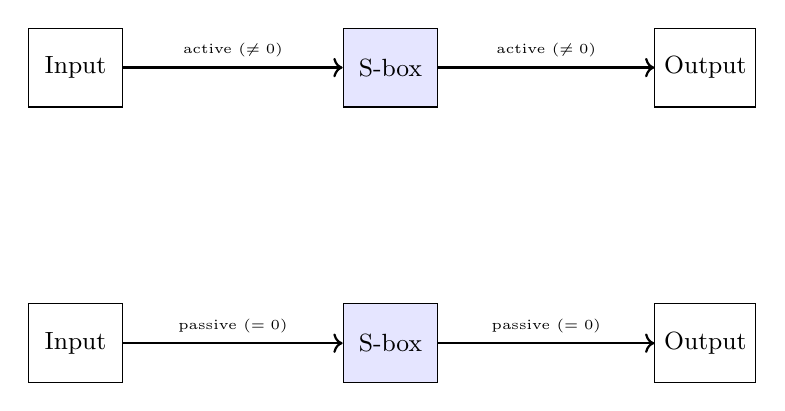
\begin{tikzpicture}[node distance=2cm, every node/.style={font=\small}]
  % Input/output boxes
  \node (input) [draw, minimum width=1.2cm, minimum height=1cm] {Input};
  \node (sbox) [draw, rectangle, right of=input, xshift=2cm, minimum width=1.2cm, minimum height=1cm, fill=blue!10] {S-box};
  \node (output) [draw, right of=sbox, xshift=2cm, minimum width=1.2cm, minimum height=1cm] {Output};

  % Arrows
  \draw[->, thick] (input) -- node[above] {\tiny active ($\neq 0$)} (sbox);
  \draw[->, thick] (sbox) -- node[above] {\tiny active ($\neq 0$)} (output);

  % Second row
  \node (input2) [draw, below of=input, yshift=-1.5cm, minimum width=1.2cm, minimum height=1cm] {Input};
  \node (sbox2) [draw, rectangle, right of=input2, xshift=2cm, minimum width=1.2cm, minimum height=1cm, fill=blue!10] {S-box};
  \node (output2) [draw, right of=sbox2, xshift=2cm, minimum width=1.2cm, minimum height=1cm] {Output};

  \draw[->, thick] (input2) -- node[above] {\tiny passive ($= 0$)} (sbox2);
  \draw[->, thick] (sbox2) -- node[above] {\tiny passive ($= 0$)} (output2);
\end{tikzpicture}
\end{center}

\end{frame}
%---------------------------------------------------------
\section{H-representation}

%---------------------------------------------------------
\begin{frame}
\frametitle{H-representation of a Polyhedron}

The \textbf{H-representation} (half-space representation) defines a polyhedron as the intersection of a finite number of half-spaces. Each half-space is defined by a linear inequality:

\[
\mathbf{a} \mathbf{x} \leq b
\]

\begin{itemize}
    \item $\mathbf{a} \in \mathbb{R}^n$: vector of coefficients.
    \item $\mathbf{x} \in \mathbb{R}^n$: vector of variables.
    \item $b \in \mathbb{R}$: scalar constant.
\end{itemize}
\end{frame}
%---------------------------------------------------------
\begin{frame}{H-representation of a Polyhedron}
\vspace{0.3cm}
\textbf{Example:} A 2D polygon defined by the intersection of 4 half-spaces:

\begin{center}
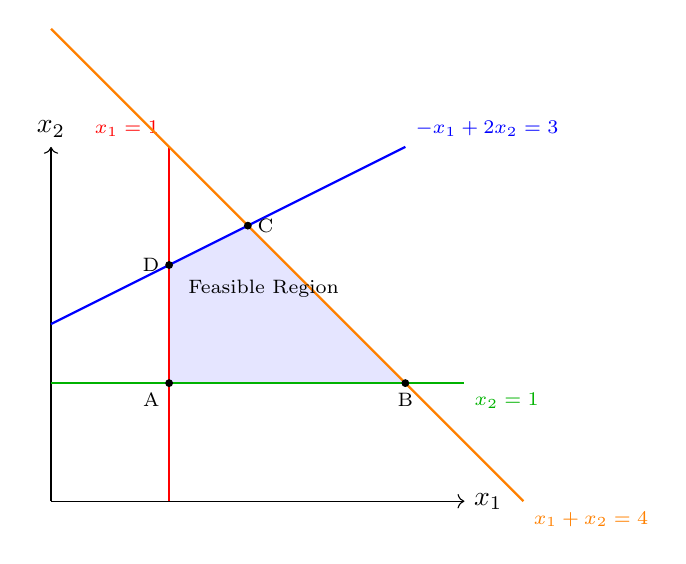
\begin{tikzpicture}[scale=1.5]

% Feasible region (corrected)
\fill[blue!10] 
    (1,1) -- % A
    (3,1) -- % B
    (1.6667,2.3333) -- % C
    (1,2) -- % D
    cycle;

% Axes
\draw[->] (0,0) -- (3.5,0) node[right] {$x_1$};
\draw[->] (0,0) -- (0,3) node[above] {$x_2$};

% Constraint lines
\draw[thick,red] (1,0) -- (1,3) node[above left] {\scriptsize $x_1 = 1$};
\draw[thick,green!70!black] (0,1) -- (3.5,1) node[below right] {\scriptsize $x_2 = 1$};
\draw[thick,orange] (0,4) -- (4,0) node[below right] {\scriptsize $x_1 + x_2 = 4$};
\draw[thick,blue] (0,1.5) -- (3,3) node[above right] {\scriptsize $-x_1 + 2x_2 = 3$};

% Feasible region label
\node at (1.8,1.8) {\scriptsize Feasible Region};

% Points
\filldraw[black] (1,1) circle (0.8pt) node[below left] {\scriptsize A};
\filldraw[black] (3,1) circle (0.8pt) node[below] {\scriptsize B};
\filldraw[black] (1.6667,2.3333) circle (0.8pt) node[right] {\scriptsize C};
\filldraw[black] (1,2) circle (0.8pt) node[left] {\scriptsize D};

\end{tikzpicture}
\end{center}

\end{frame}




%---------------------------------------------------------
\begin{frame}
    \frametitle{H-representation}
    This representation is integral to the MILP modeling of
    block ciphers as it encapsulates the constraints from the cipher’s operations, including
    the behavior of S-boxes, linear layers, and key additions.
    In the context of cryptanalysis, using the H-representation allows complex
    relationships between variables to be expressed linearly, enabling MILP solvers to
    explore the solution. 
\end{frame}
%---------------------------------------------------------
\begin{frame}
    \frametitle{H-representation example}
    Consider linear function L which takes 6 bit input, 6 bit output and computed as:
\begin{center}
    $L(a,b,c)=(a \oplus b , a \oplus c , b \oplus c ) \text{ where a,b.c are 2 bit values}  $
\end{center}
H-representation of this function can be found in 2 steps with using  Sagemath polyhedra library. \cite{sage}
\end{frame}
%---------------------------------------------------------
%---------------------------------------------------------
\begin{frame}
    \frametitle{H-representation example}
    \begin{enumerate}
    \item We scan the outputs for all possible inputs and give a value of 0 if the output value is 0 and 1 if it is different from zero. Possible input and output values of the $L$ function can be seen in Table \ref{tab:hreptab}.

    \item These points are given as input to the sage polyhedra library and the inequalities given in table \ref{tab:h-repineq} are obtained.
    
\end{enumerate}

    
\end{frame}
%---------------------------------------------------------
\begin{frame}
    \frametitle{H-representation example}
\begin{table}[h]
\footnotesize
\centering
\begin{tabular}{|c|c|}
\hline
\textbf{Input Differences} & \textbf{Output Differences} \\ \hline
0 0 0 & 0 0 0 \\ \hline
0 0 1 & 0 1 1 \\ \hline
0 1 0 & 1 0 1 \\ \hline
0 1 1 & 1 1 0 \\ \hline
0 1 1 & 1 1 1 \\ \hline
1 0 0 & 1 1 0 \\ \hline
1 0 1 & 1 0 1 \\ \hline
1 0 1 & 1 1 1 \\ \hline
1 1 0 & 0 1 1 \\ \hline
... & ... \\ \hline
1 1 1 & 1 0 1 \\ \hline
1 1 1 & 1 1 0 \\ \hline
1 1 1 & 1 1 1 \\ \hline
\end{tabular}
\caption{Input and Output Differences of $L$ function}
\label{tab:hreptab}
\end{table}
    
\end{frame}
%---------------------------------------------------------
\begin{frame}
    \frametitle{H-representation example}
\begin{table}[h]
\footnotesize
\centering
\begin{tabular}{|c|l|}
\hline
\textbf{No.} & \textbf{Inequality} \\ \hline
1  & $(0, 0, -1, 0, 0, 0) x + 1 \geq 0$ \\ \hline
2  & $(0, -1, 0, 0, 0, 0) x + 1 \geq 0$ \\ \hline
3  & $(-1, 0, 0, 0, 0, 0) x + 1 \geq 0$ \\ \hline
4  & $(0, 0, 0, -1, 0, 0) x + 1 \geq 0$ \\ \hline
5  & $(0, 0, 0, 0, -1, 0) x + 1 \geq 0$ \\ \hline
6  & $(0, 0, 0, 0, 0, -1) x + 1 \geq 0$ \\ \hline
7  & $(0, -1, 1, 0, 0, 1) x + 0 \geq 0$ \\ \hline
8  & $(0, 0, 0, -1, 1, 1) x + 0 \geq 0$ \\ \hline
... & ... \\ \hline
18 & $(-1, 1, 0, 1, 0, 0) x + 0 \geq 0$ \\ \hline
19 & $(1, -1, -1, 1, 1, -1) x + 1 \geq 0$ \\ \hline
20 & $(1, -1, 0, 1, 0, 0) x + 0 \geq 0$ \\ \hline
21 & $(-1, 1, -1, 1, -1, 1) x + 1 \geq 0$ \\ \hline
22 & $(-1, -1, 1, -1, 1, 1) x + 1 \geq 0$ \\ \hline
\end{tabular}
\caption{H-representation of $L$ function}
\label{tab:h-repineq}
\end{table}
    
\end{frame}
%--------------------------------------------------------
\section{Differential cryptanalysis model with MILP}

%---------------------------------------------------------
\begin{frame}
\frametitle{Differential Cryptanalysis Model Using MILP}

The ITUbee algorithm has a Feistel structure, so we represent the input as two variables, \( R0 \) and \( R1 \), each modeled as binary variables indicating activity status. 

In the MILP model, after each operation in the cipher, we introduce new binary variables whenever a byte’s activity status can change—i.e., an active byte may become passive or vice versa. 

However, the S-box operation does not alter the activity status of a byte: if the input byte is active, the output byte remains active, and if inactive, it remains inactive. Therefore, no new binary variables are introduced after S-box layers.

\end{frame}

%---------------------------------------------------------
\begin{frame}
\frametitle{Differential cryptanalysis model with MILP}
   L operations are changes the active bytes so after them we define new variable. XOR operation changes active byte if it XOR two binary variables. In differential cryptanalysis we do not give active values to the keys therefore key xor's does not change the active byte. Skech of the 1 round modelling can be seen in the Figure \ref{fig: ITUbeeDif}. 

\begin{figure}[!ht]
\footnotesize
\centering
\resizebox{1\textwidth}{!}{%
\begin{circuitikz}
\tikzstyle{every node}=[font=\small]
\node [font=\small] at (6,15) {R0};
\node [font=\small] at (6,14) {R1};
\draw [->, >=Stealth] (6.5,14.5) -- (12.5,14.5);
\node [font=\small] at (13,15) {R2};
\node [font=\small] at (13,14) {R3};
\node [font=\small,color={rgb,255:red,221; green,19; blue,19}] at (9.5,15) {XOR};
\node [font=\small, color={rgb,255:red,221; green,19; blue,19}] at (9.5,14) {L operation};
\end{circuitikz}
}%

\label{fig:my_label}
\end{figure}

\end{frame}
%---------------------------------------------------------
\begin{frame}
\footnotesize
\frametitle{Differential cryptanalysis model with MILP}
\begin{figure}[!ht]
\centering
\resizebox{1\textwidth}{!}{%
\begin{circuitikz}
\tikzstyle{every node}=[font=\large]
\node [font=\large] at (2.5,16) {R1};
\draw (2.5,15.5) to[short] (2.5,14.5);
\draw  (2.5,14) circle (0.5cm);
\draw [short] (2.5,13.5) -- (2.5,11.5);
\draw [->, >=Stealth] (2.5,11.5) -- (4,11.5);
\draw  (4,12) rectangle  node {\large SLS} (5.25,11);
\draw [->, >=Stealth] (5.25,11.5) -- (6.5,11.5);
\draw [short] (2.5,14.5) -- (2.5,13.5);
\draw [short] (2,14) -- (3,14);
\draw  (7,11.5) circle (0.5cm);
\draw [->, >=Stealth] (7.5,11.5) -- (8.75,11.5);
\draw  (8.75,12) rectangle  node {\large L} (10,11);
\draw [->, >=Stealth] (10,11.5) -- (11.5,11.5);
\draw  (11.5,12) rectangle  node {\large SLS} (12.75,11);
\draw [->, >=Stealth] (12.75,11.5) -- (14.5,11.5);
\draw  (15,11.5) circle (0.5cm);
\node [font=\large] at (15,16) {R0};
\draw (15,15.5) to[short] (15,14.5);
\draw  (15,14) circle (0.5cm);
\node [font=\large] at (3,11.75) {};
\draw [short] (15,13.5) -- (15,12);
\draw [short] (6.5,11.5) -- (7.5,11.5);
\draw [short] (7,12) -- (7,11);
\draw [short] (14.5,11.5) -- (15.5,11.5);
\draw [short] (15,12) -- (15,11);
\draw [short] (14.5,14) -- (15.5,14);
\draw [short] (15,14.5) -- (15,13.5);
\draw [short] (15,11) -- (15,10.25);
\draw [short] (2.5,11.5) -- (2.5,10.25);
\draw [short] (2.5,10.25) -- (15,8.25);
\draw [short] (15,10.25) -- (2.5,8.25);
\node [font=\large] at (1.5,14) {KL};
\node [font=\large] at (16,14) {KR};
\node [font=\large] at (7,12.5) {KR};
\node [font=\large] at (3.25,12) {R1};
\node [font=\large] at (5.75,12) {R1a};
\node [font=\large] at (8,12) {R1a};
\node [font=\large] at (10.75,12) {R1b};
\node [font=\large] at (13.75,12) {R1c};
\node [font=\large] at (15.5,10.5) {R2};
\node [font=\large] at (2.5,8) {R2};
\node [font=\large] at (15,8) {R1};
\end{circuitikz}
}%
\caption{ITUbee  MILP differential cryptanalysis sketch}
\label{fig: ITUbeeDif}
\end{figure}

\end{frame}
%---------------------------------------------------------
\begin{frame}{Differential Cryptanalysis Model with MILP}

\begin{itemize}
    \item In MILP-based differential cryptanalysis, our goal is to find the best differential characteristic by minimizing the number of active S-boxes.
    \item We model binary variables before and after each S-box and minimize their sum to find the characteristic with the lowest activity.
    \item The ITUbee block cipher uses the AES S-box~\cite{dworkin2001advanced}, which has a maximum differential probability of $2^{-6}$.
\end{itemize}

\begin{block}{Model Output (3 Rounds)}
\begin{itemize}
    \item The best characteristic found activates 16 S-boxes over 3 rounds.
    \item Therefore, the maximum differential probability is:
    \[
    (2^{-6})^{16} = 2^{-96}
    \]
\end{itemize}
\end{block}

\end{frame}
%---------------------------------------------------------
\begin{frame}{Differential Cryptanalysis Model with MILP}

\begin{itemize}
    \item A differential characteristic with probability $2^{-96}$ is too low to be useful for a practical attack.
    \item This result implies that 3 rounds of the ITUbee cipher are secure against differential cryptanalysis.
    \item Our findings are consistent with those reported in~\cite{karakocc2013itubee}.
\end{itemize}

\begin{block}{Characteristic Table}
The best differential characteristic found by the MILP model is shown in Table~\ref{tab:MILPcharDif}.
\end{block}

\end{frame}

%---------------------------------------------------------
\begin{frame}
\frametitle{Differential cryptanalysis model with MILP}
\begin{table}[H]
    \footnotesize
    \centering
    \begin{tabular}{|c|c|c|}
        \hline
        \textbf{Stage} & \textbf{Binary Index} & \textbf{Characteristic} \\
        \hline
        1. round  & R1 & \{0: 0.0, 1: 0.0, 2: 0.0, 3: 0.0, 4: 1.0\} \\
        input      & R0 & \{0: 0.0, 1: 0.0, 2: 0.0, 3: 0.0, 4: 0.0\} \\
        \hline
        1. round  & R1a & \{0: 1.0, 1: 0.0, 2: 0.0, 3: 1.0, 4: 1.0\} \\
        middle values   & R1b & \{0: 0.0, 1: 1.0, 2: 1.0, 3: 0.0, 4: 1.0\} \\
                   & R1c & \{0: 0.0, 1: 0.0, 2: 0.0, 3: 0.0, 4: 1.0\} \\
        \hline
        2. round& R2 & \{0: 0.0, 1: 0.0, 2: 0.0, 3: 0.0, 4: 1.0\} \\
        input      & R1 & \{0: 0.0, 1: 0.0, 2: 0.0, 3: 0.0, 4: 1.0\} \\
        \hline
        2. round & R2a & \{0: 1.0, 1: 0.0, 2: 0.0, 3: 1.0, 4: 1.0\} \\
        middle values  & R2b & \{0: 0.0, 1: 1.0, 2: 1.0, 3: 0.0, 4: 1.0\} \\
                   & R2c & \{0: 0.0, 1: 0.0, 2: 0.0, 3: 0.0, 4: 1.0\} \\
        \hline
        3. round  & R3 & \{0: 0.0, 1: 0.0, 2: 0.0, 3: 0.0, 4: 0.0\} \\
        input     & R2 & \{0: 0.0, 1: 0.0, 2: 0.0, 3: 0.0, 4: 1.0\} \\
        \hline
        3. round  & R3a & \{0: 0.0, 1: 0.0, 2: 0.0, 3: 0.0, 4: 0.0\} \\
        middle values   & R3b & \{0: 0.0, 1: 0.0, 2: 0.0, 3: 0.0, 4: 0.0\} \\
                   & R3c & \{0: 0.0, 1: 0.0, 2: 0.0, 3: 0.0, 4: 0.0\} \\
        \hline
        4. round & R4 & \{0: 0.0, 1: 0.0, 2: 0.0, 3: 0.0, 4: 1.0\} \\
        input    & R3 & \{0: 0.0, 1: 0.0, 2: 0.0, 3: 0.0, 4: 0.0\} \\
        \hline
    \end{tabular}
    \caption{Best 3 round differential characteristic of ITUbee algorithm}
    \label{tab:MILPcharDif}
\end{table}

\end{frame}
%---------------------------------------------------------

\section{References}

%---------------------------------------------------------
\begin{frame}
\frametitle{References}

\printbibliography

\end{frame}
%---------------------------------------------------------



\end{document}